\section{CUDA programming model}
CUDA is a general-purpose heterogeneous parallel computing platform and programming model that uses the parallel compute engine in NVIDIA GPUs to perform many complex computations in a more efficient way \cite{ProfessionalCUDA}. NVIDIA GPUs are accessible through CUDA platform, CUDA is accessible through CUDA-accelerated libraries(NVIDIA Performance Primitives), compiler directives, APIs (Application Programming Interfaces), and extensions to standard programming languages such as C, C++, Fortran, and Python.
\paragraph*{} CUDA C is inherited most of the ANSI C attributes and contains the handful of features to handle parallel programming on NVIDIA GPUs. The unique feature of CUDA is its scalable programming model, that enables programs to transparently scale their parallelism to GPUs with varying numbers of cores. There are two driver APIs in CUDA to manage device activities.
\begin{itemize} 
\item CUDA driver API
\item CUDA Runtime API
\end{itemize}
As shown from the Figure \ref{Figure 1.2}, the device code and host code are separately compiled with the suitable compilers. The host code is compiled by ANSI C compilers, and NVIDIA CUDA \textit{nvcc} compiler compiles the device code. The device code contains kernels which are CUDA C extensions for data parallel functions. During the link stage CUDA runtime libraries will be added for kernel procedure calls and explicit GPU usage. Programming models act as a bridge between an application and its implementation on available computer architecture\cite{ProfessionalCUDA}. The CUDA programming model provides special features like organizing threads, accessing GPU memory, etc.

\paragraph*{} Parallel computation can be viewed in different levels for a programmer, as described below
\begin{description}
\enlargethispage{-\baselineskip}
\item [Domain level] \hfill \break At this level, the main concern is to decompose data and functions in an algorithm such that the problem is solved efficiently and correctly in a parallel environment. The motion de-blur algorithm illustrated in this work contains a handful of parallel operations, all these are exposed when the Domain level inspection is performed. The motion deblur algorithm includes image gradient , FFT calculation, IFFT calculation, deconvolution operations, which are targeted portions for parallel computing.
\item [Logic level] \hfill \break When programming for a problem in a parallel environment, our focus is to organise concurrent threads to solve the problem. In C parallel programming this can be done by using \textit{pthreads} or \textit{openMP} techniques.
\item[Hardware level] \hfil \break 
The efficient mapping of threads to the available cores gives the best performance in parallel processing. In CUDA the thread mapping is done implicitly by considering the programmer's view of parallelism. So, a programmer can specify the amount of threads he want to use.
\end{description}
\section{CUDA development cycle}
 For the purpose of improving application performance, NVIDIA has suggested a development cycle \cite{apod}. The development cycle is a repetitive process where refinement to the previous implementation happens and it makes the application perform better. It contains four stages, they are Asses, Parallelize, Optimise and Deploy as shown in the Figure \ref{Figure:2.1}.
\begin{figure}[h!]
  \centering
  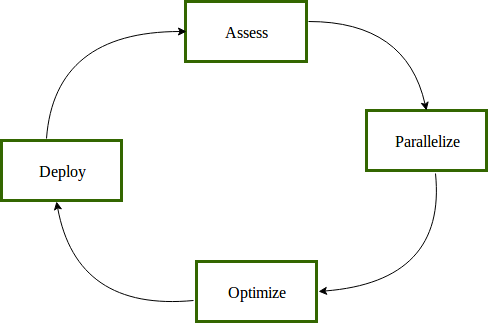
\includegraphics[width=0.75\textwidth]{cudaDevCycle.png}
  \caption{CUDA development cycle \cite{apod}}
  \label{Figure:2.1}
\end{figure}
\subsection{Assess}
In this stage, algorithm or code is analysed such that we come to know the most time-consuming parts(hot spots). Targeting specific portions of the algorithm makes easy work around to start developing the application. In case working with the already developed unoptimized code, then time profiling the code gives the suitable parts to parallelize.
\subsection{Parallelize}
After Identifying the portions for GPU implementation, the next task is to identify the parallelism in those portions and starting a design task for implementation. It is a very crucial stage and challenges the developer.
\subsection{Optimize}
The performance of the application can further be improved by optimising the parallel implementation. This can be a repetitive process of finding an opportunity, applying the optimisation, testing the optimisation and checking the speed achieved and repeating the same process again. Optimisation can be overlapped computation and data transfers, coalesced memory access, reducing global memory access, etc.
\subsection{Deploy}
Before finding more hot spots in the algorithm or code, the partially parallelized code will be considered for production. This makes the developer risk free and profits the user for his investment.
\section{CUDA memory hierarchy}
One of the unique characteristics of CUDA is its exposed memory architecture, which enables users to use the suitable memory for their application. In CPU memory hierarchy the L1 and L2 caches has very less memory transaction cost. But these memories are not user programmable. CUDA has a programmable memory structure, Figure \ref{Figure:2.2} illustrates different memories on an NVIDIA GPU.
\begin{figure}[h!]
  \centering
  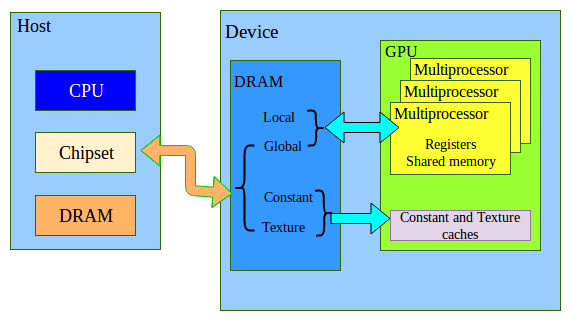
\includegraphics[width=\textwidth]{CUDA_MEM_hierarchy.png}
  \caption{NVIDIA GPU memory model \cite{ProfessionalCUDA}}
  \label{Figure:2.2}
\end{figure}
The programmable memories in NVIDIA GPUs using CUDA are\cite{ProfessionalCUDA},
\begin{enumerate}
\enlargethispage{-\baselineskip}
\item \textbf{Registers}
\begin{itemize}
\item Registers are fastest memory in the GPU, a variable declared in a kernel is expected to store in a register,and these are private to each thread.
\item The life time is the kernel execution time. The number of register variables used in a kernel effects the occupancy of the kernel. The kernel occupancy is the resource utilization of that kernel.
\item  If a kernel uses more number of registers than the hardware limit, the additional registers will spill over to local memory. The compiler option \textit{-maxregcount} will limit the maximum number of registers used by all kernel.
\end{itemize} 
\item \textbf{Shared memory}
\begin{itemize}
\item Shared memory is on-chip, it's memory access cost very low when compared with local and global memory. The CPU L1 cache and shared memory are comparable but shared memory is programmable.
\item The shared memory is local to each thread block and enables inter thread communication. Shared memory is limited to each SM, so over usage of it limits number of active warps.
\end{itemize}
\item \textbf{Local memory}
\begin{itemize}
\item The register variables which can not have a register space to be accommodated are eligible to occupy in a local memory.
\item Local arrays referenced with indices whose values cannot be determined at compile-time will be allocated in local memory.
\item Variables mapped to local memory will reside in the global memory, so the memory access is more costly (high latency and low bandwidth).
\end{itemize}
\item \textbf{Constant memory}
\begin{itemize}
\item Constant memory resides in a device memory and is cached to constant cache in each SM. Constant memory is accessible to all kernels,only a 64KB of constant memory is allowed to declare.
\item Constant memory is a read only memory.
\end{itemize}
\item \textbf{Texture memory}
\begin{itemize}
\item Texture memory resides in device memory and will be cached to read only cache in each SM.
\item It is optimized for 2D spatial locality, so the threads in a warp that use texture memory can achieve best performance. It is used for window operations on an image such as convolution and filtering.
\end{itemize}
\item \textbf{Global memory}
\begin{itemize}
\item This is the highest latency memory and it is available throughout the entire application. This is the most commonly used memory.
\item Global memory resides in the device memory and it is accessible via 32-bit, 64-bit,128-bit transactions.
\item To get the optimal performance of the application the memory transactions should be aligned properly.
\end{itemize}
\end{enumerate}
\section{Memory management in CUDA}
CUDA kernels operate only on the device memory. CUDA runtime provides several functions to manage memory effectively as shown in Table  \ref{Memory management in CUDA}. Each of the below functions listed in Table \ref{Memory management in CUDA} returns an error code after invocation which is useful to handle errors effectively.
\begin{table}[h!]
\centering
\begin{tabular}{ |c|c| }
\hline
\textbf{CUDA C functions} & \textbf{Description} \\
\hline
cudaMalloc & Allocates memory on device(Global memory) \\  
\hline
cudaMemcpy & Transfers memory across host and device \\	
\hline
cudaMemset & Sets the memory with a given value \\
\hline
cudaFree & Deallocates the device memory \\
\hline
\end{tabular}
\caption{CUDA APIs for Memory management}
\label{Memory management in CUDA}
\end{table}
All the functions are called from host, but they manage memory at device. So CPU has full control over device, as can be seen from Figure \ref{Memory management}.

\begin{figure}[h!]
  \centering
  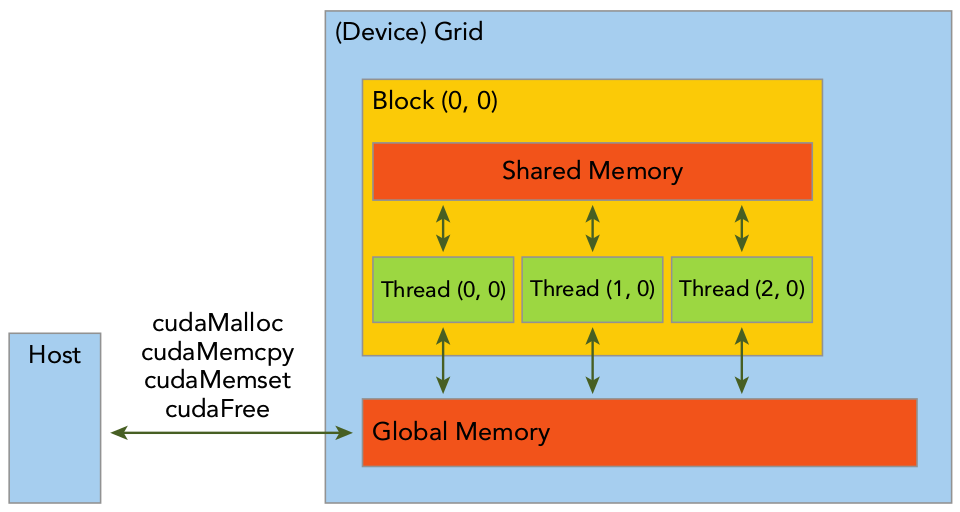
\includegraphics[width=\linewidth]{cudaMemMangement.png}
  \caption{CUDA APIs to manage global memory \cite{ProfessionalCUDA}}
  \label{Memory management}
\end{figure}
\section{Organizing threads in CUDA}
When host invokes a kernel function, a large number of threads are created on device\cite{ProfessionalCUDA}. These threads work on the statements specified in the kernel. CUDA follows a two level thread hierarchy abstraction which provides users to organize threads efficiently. The two stage thread hierarchy is decomposed into block of threads and grids of blocks, as shown in the Figure \ref{Thread-block hierarchy}. All the Threads created in a single kernel launch are called a grid, and access the same global memory. A grid is made up of many thread blocks, a thread block is a group of threads, and in the blocks threads cooperate with each other using shared memory or by using block level synchronization.\paragraph*{}Each thread is distinguished using two unique 	coordinates, they are \textit{blockIdx} and \textit{threadIdx} which are assigned to each thread by CUDA runtime. The \textit{blockIdx} and \textit{threadIdx} are of type \textit{uint3} which is derived from basic integer type and comprises three unsigned integers. These three components are accessible with x,y,z extensions as,
\begin{itemize}
\item \textit{blockIdx.x}
\item \textit{blockIdx.y}
\item \textit{blockIdx.z}
\item \textit{threadIdx.x}
\item \textit{threadIdx.y}
\item \textit{threadIdx.z}
\end{itemize}
The grid and block dimensions are specified by the implicit variables \textit{blockDim} and \textit{gridDim} which are of type \textit{dim3}. When defining a variable of type \textit{dim3 }, any component left unspecifi ed is initialized to 1. These are accessible through its x, y, and z fields as,
\begin{itemize}
\item \textit{blockDim.x}
\item \textit{blockDim.y}
\item \textit{blockDim.z}
\end{itemize}
\begin{figure}[h!]
  \centering
  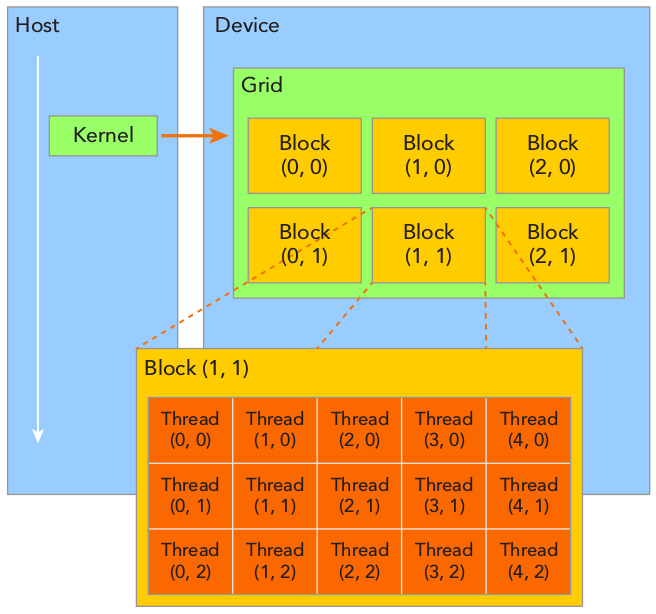
\includegraphics[width=0.75\linewidth]{thread-block.png}
  \caption{Thread-block hierarchy in CUDA \cite{ProfessionalCUDA}}
  \label{Thread-block hierarchy}
\end{figure}
Setting of block and grid sizes is crucial, first we will decide the block size. The grid dimension are calculated based on the input data size and block size. The block size depends on the performance characteristics of the kernel and on the available GPU resources.
\section{CUDA programming structure}
The key element in the CUDA programming is the kernel which is the part of the code that runs on the GPU. Implicitly the CUDA manages scheduling the kernels on GPU threads. The main aspect in CUDA programming is memory access, the memory on the CPU is explicitly copied to the GPU memory. The CPU memory is termed as host memory where as GPU memory is called as device memory.\paragraph*{}The host operates independently to the device,the control is returned after a kernel is launched, CPU can perform the sequential tasks. The GPU and CPU activities can overlapped since most of the GPU calls are asynchronous. The host code is in ANSI C and device code is in CUDA C, the different types can be integrated into a single file or can be put into a different files. A typical CUDA program flow is given below,
\begin{itemize}
\item Allocate Memory on the device
\item Copy data from CPU to GPU
\item Invoke kernels to operate on the data available in the GPU memory
\item Copy data back from GPU memory to CPU memory
\item Deallocate device memory
\end{itemize}
%\subsection{\textbf{CUDA sample program}}
The program in Appendix A illustrates a matrix addition, two matrices of same size are taken and are added. All the elements in one matrix are added to respective elements in another matrix in parallel with the help of parallel threads using CUDA. The number of parallel threads used in this sample program are equal to the size of matrix, so each thread operates on each addition operation. The matrix addition program performs matrix addition on GPU and verifies the same on CPU. When we profile the above program the NVIDIA GeForce GT640 GPU takes around 0.25 milli seconds (excluding memory copies) where as Intel i5 CPU@3.0GHz takes 1.39 milli seconds. For now we are not considering the latency for memory copies to and fro from GPU, anyway these latencies will be hidden when we are working with large data.\paragraph*{}The computer vision and image processing algorithms works on large data as the input being is an image(colour or gray), so GPU enabled environment is most suitable to implement these algorithms. In this work Adaptive Image contrast enhancement, motion deblur algorithm are implemented using CUDA C language on NVIDIA GeForce GT640 GPU. The Autonomous drive algorithms like temporal denoising and fog rectification with denoising are implemented using multi-core CPU(ARM A57). And stereo disparity algorithm is also implemented to extract the hidden capabilities of GPU like CUDA intrinsics, streams, etc.

\section{Multi-core CPU programming}
The multi-core CPU programming is available for the user through the software library \textit{posix threads}. Threads will be created and are mapped to the CPU cores. Semaphores are used for inter thread communication. The fog rectification and temporal denoising are implemented using this programming model.


%\end{document}